\documentclass[preprint,review,12pt]{elsarticle}
\usepackage[T1]{fontenc}
\usepackage[utf8]{inputenc}
\usepackage{lmodern}
\usepackage{amsmath,amssymb,booktabs,array}
\usepackage{graphicx}
\usepackage{float}
\usepackage{microtype}
\usepackage{setspace}
\usepackage[a4paper,margin=25mm]{geometry}
\usepackage[hidelinks]{hyperref}
\journal{Pattern Recognition}
\makeatletter
\let\ps@pprintTitle\ps@plain
\gdef\@blstr{1.655}
\makeatother
\doublespacing
\graphicspath{{figures/}}
\setlength{\emergencystretch}{2em}
\clubpenalty=10000
\widowpenalty=10000
\displaywidowpenalty=10000
\renewcommand{\topfraction}{0.9}
\renewcommand{\bottomfraction}{0.8}
\renewcommand{\textfraction}{0.08}
\renewcommand{\floatpagefraction}{0.85}
\newcommand{\ctc}{\mathrm{CTC}}
\newcommand{\att}{\mathrm{att}}
\newcommand{\sg}{\operatorname{sg}}
\newcommand{\KL}{\operatorname{KL}}
\begin{document}
\begin{frontmatter}
\title{Fragment-Mixed Continuation for Cross-Corpus Visual Speech Recognition}
\author{Anonymous authors}
\begin{abstract}
Improving a visual speech recognizer on its training corpus need not improve
transcription of an unfamiliar video collection. We study temporal supervision
granularity during source-only continuation, preserving the architecture and
whole-utterance inference. Fragment-mixed continuation alternates complete
utterances with short, transcript-labelled views of the same videos. Comparisons
match initialization, source-clip order and 6,000 optimizer updates. On 1,167
ViCocktail clips after VLR continuation, fixed-time mixing reduces common-decoder
word error rate (WER) by 3.41 and 3.17 percentage points across two seeds.
A separate matched comparison obtains 67.37\% WER with full-only continuation,
63.85\% with fixed-time mixing and 63.39\% with whole-word mixing. Replacing the
scheduled full views with additional whole-word fragments raises destination
WER to 70.72\% and source WER to 44.84\%, compared with 38.61\% source WER for
whole-word mixing. Increased deletions outweigh fewer substitutions and insertions.
Retaining full-utterance presentations therefore benefits both populations in
this fixed-budget comparison. Relative to full-only continuation, the two mixed
states still incur source costs of 0.55 and 0.58 WER points. The fixed-time
transfer gain persists at 3.46 points after component-wise token normalization.
In LRS2-to-WildVSR transfer, mixing gives up 1.46 source WER points without a
clear destination gain. These results support mixed temporal supervision in
the studied Vietnamese continuation setting, while showing that its value depends
on the training regime and must be assessed jointly on source and destination.
\end{abstract}
\begin{keyword}
Visual speech recognition \sep Lip reading \sep Cross-corpus transfer \sep
Fragment-mixed continuation \sep Temporal supervision
\end{keyword}
\end{frontmatter}

\section{Introduction}
Visual speech recognition (VSR) recovers linguistic content from visible mouth
movements. Large-scale supervised learning has substantially improved benchmark
accuracy \cite{shillingford2019large,ma2023autoavsr}, yet strong performance on a
training corpus does not ensure reliable transcription of a different video
collection \cite{djilali2024wildvsr}. For an existing recognizer, a practical
question is how to reuse labelled source videos before deployment elsewhere.
We ask whether changing the temporal scope of supervision during source-only
continuation improves complete destination transcripts, and what it gives up
on the source corpus.

Complete utterances supply extensive visual and linguistic context. Short views
contain fewer neighboring frames and shorter target sequences, changing both
the available evidence and the optimization problem. A temporal cut can also
remove visual evidence for a boundary word retained in the target. These changes
make short-view supervision a testable intervention, rather than an assumed
improvement over complete clips.

Our initial formulation, fragment-mixed continuation (FM), alternates complete
source utterances with fixed-duration, transcript-labelled fragments of the same
videos. Fragment targets contain the transcript units overlapping each interval.
Only the training presentations change: the recognizer keeps its architecture
and ordinary whole-utterance decoding. No fragment selection, timestamp estimation
or prediction merging is required at inference, and no additional source videos
are introduced.

Full-clip continuation (FC) provides the comparison under the same initialization,
source-clip order and 6,000 optimizer updates. A common decoder compares fitted
states; development-selected decoders additionally describe calibrated systems.
Equal numbers of updates and presentations do not imply equal frame or token
exposure. We measure these exposures and retain the native objective, treating
the recipe as a complete intervention under an update budget rather than
attributing its effect to one regularization mechanism.

Two corpus pairs expose different outcomes. In VLR-to-ViCocktail transfer,
FM reduces common-decoder WER by 3.41 and 3.17 percentage points across two
seeds. In LRS2-to-WildVSR transfer, it gives no clear aggregate gain. The seed-17
source assessment shows that FM improves over each initializer but retains less
of FC's source improvement in both settings. The Vietnamese transfer gain thus
accompanies a source cost. Differences in initialization, training coverage,
repetition and calibration prevent attributing the contrast between corpus pairs
to language alone.

Temporal cropping and mixed-length training are established in lip reading
\cite{martinez2020lipreading,prajwal2022subword}. A separate matched comparison
therefore includes conventional whole-word mixing, which improves transfer and
outperforms fixed-time mixing by 0.459 WER points. A paired token-normalized loss
control retains the fixed-time gain. The whole-word short-only control further
tests the contribution of scheduled full-clip presentations, using the same
source order and unchanged whole-utterance assessment. Together, these controls
test how temporal schedule, fragment labelling and loss reduction shape source
retention and destination recognition.
The short-only state is worse than whole-word mixing by 7.328 destination WER
points and 6.238 source points, with substantially more deletions. Retaining
scheduled full views is therefore beneficial in this comparison; increasing
the proportion of short supervision does not monotonically improve transfer.

Two same-target controls restore neighboring pixels or supply predictions
informed by the complete video. Neither improves on FM in the Vietnamese
comparison. Their edit-error profiles show that improved visual coverage or
fewer substitutions can be offset by additional deletions, motivating assessment
of the complete output sequence.

The paper contributes three results:
\begin{itemize}
 \item A controlled study of source-only short-view continuation under matched
 update budgets, with unchanged whole-utterance recognition at deployment.
 \item A decoder-controlled comparison across two corpus pairs, including a
 two-seed Vietnamese transfer gain and joint source/destination assessment
 that identifies where the intervention does not improve recognition.
 \item Comparisons of temporal schedule, crop labelling, loss reduction and
 same-target context, supported by edit-error and exposure measurements.
\end{itemize}
Together, these results characterize when mixed temporal supervision improves
transfer, how retaining full utterances contributes, and the source-retention
cost of the resulting continuation strategy.

\section{Related work}
\subsection{Learning visual speech representations}
Continuous lip reading combines spatial analysis of the mouth with temporal and
linguistic modeling. Sentence-level systems established the importance of learning
over variable-length visual sequences \cite{chung2017lipreading,afouras2022deep}.
Large-scale supervised recognition subsequently expanded the available training
resources \cite{shillingford2019large}. Auto-AVSR uses automatically generated
labels to exploit additional audiovisual collections \cite{ma2023autoavsr}, while
AV-HuBERT learns audiovisual representations through masked cluster prediction
\cite{shi2022avhubert}. These approaches address representation quality and scale.
Our experiments instead start from existing language-specific recognizers and
study how the presentation of supervision affects transfer under a fixed update
budget, using the same visual backbone and source-video collection.

The recognizers considered here use a hybrid CTC/attention formulation
\cite{graves2006ctc,watanabe2017hybrid}. The two output components provide useful
controls because changing their relative decoding weight can change substitutions,
deletions and insertions without changing the trained model. Accordingly, we report
both a decoder selected for each checkpoint on development data and a common
decoder. Together, these comparisons distinguish the performance of the tuned
system from the effect observed under a shared decoding rule.

\subsection{Temporal crops and short-sequence supervision}
Training on shorter sequences is not new to lip reading. Early sentence-level work
used a progression in sequence difficulty \cite{chung2017lipreading}.
Martinez et al. vary temporal context around an intact target word, improving
robustness to frame removal in isolated-word recognition
\cite{martinez2020lipreading}. Their BGRU comparison also illustrates that
robustness and unperturbed accuracy can change in different directions.
Prajwal et al. train with consecutive-word subsequences and compare increasing
subsequence length with using different lengths together
\cite{prajwal2022subword}. Their study is particularly relevant because it shows
that mixed temporal scales provide an established augmentation baseline. We build
on this setting to examine transfer under matched continuation budgets and
whole-utterance evaluation on a different corpus.

Recent word-level work also examines temporal information and augmentation.
InfoSyncNet combines temporal modeling with time masking, mixup and word-boundary
indicators, reporting different time-masking effects on LRW and LRW1000
\cite{xue2025infosyncnet}. These experiments retain an isolated-word recognition
task. FM instead changes both the visual interval and its transcript during
continuation, then evaluates complete utterances on a destination corpus.

The specific setting examined here differs in two respects. The fragment is defined
by a fixed time interval rather than a fixed number of complete words. Its label
contains any transcript unit that overlaps the interval, so boundary words can
remain in the target despite incomplete visual coverage. Moreover, evaluation
uses complete utterances from a different corpus, rather than the same fragment
task used during continuation. These choices create a testable question about the
interaction between context availability and transfer. We examine this fixed-time
formulation through paired context-restoration controls and a direct comparison
with conventional word-aligned fragments. The latter tests the crop choice within
our continuation protocol; it is not a reimplementation of Prajwal et al.'s
architecture or complete training pipeline. The distinction from prior work lies
in the joint assessment of whole-utterance transfer, source performance and
decoder dependence after continuation, rather than in temporal cropping alone.

\subsection{Contextual targets and consistency learning}
Self-distillation provides a way to use information that is available during
training but absent from a particular input view. For example, data2vec predicts
contextual representations of the full input from a masked view
\cite{baevski2022data2vec}. Closer to the recognition objective, CR-CTC encourages
agreement between framewise CTC distributions from two augmented speech views
\cite{yao2025crctc}. Its branches share transcript supervision, with bidirectional
consistency and stop-gradient targets at corresponding time positions.

Our full-view control examines broader temporal context during fragment learning.
The current model supplies a stop-gradient CTC target from the complete video,
restricted to the fragment's time positions, while the student retains its
fragment transcript. It therefore tests contextual guidance alongside the
alternative of exposing additional context directly to the encoder. Both controls
retain ordinary whole-utterance inference. This framing connects the experiments
to established consistency learning while focusing the comparison on the context
available when learning from partial speech.

\subsection{Cross-corpus evaluation and multilingual evidence}
Speaker adaptation addresses distribution shift using examples from the intended
users. Kim et al. learn prompts from target-speaker adaptation data while
preserving the pretrained recognizer parameters \cite{kim2025prompt}. Here,
recognizer gradient updates use the continuation source; destination development
data are used only for decoder calibration where the protocol permits it.
This distinction separates source continuation from target-speaker fitting.

WildVSR was introduced to examine whether strong VSR models generalize beyond
LRS3 \cite{djilali2024wildvsr}. Its results motivate retaining an external-corpus
assessment even when source-domain validation appears satisfactory. We use WildVSR
as the English destination corpus and ViCocktail as the Vietnamese destination
\cite{nguyen2025vicocktail}. The Vietnamese source is the VLR dataset
\cite{vlr2026dataset}; English continuation uses prepared LRS2 training clips.
The two comparisons share the intervention and whole-utterance objective, but
they are distinct transfer settings with different initializations, tokenizers,
training coverage and development-data availability.

We analyze each corpus pair separately, examining training coverage, edit types
and sequence length as possible explanations for their contrasting outcomes.

\section{Fragment-mixed continuation}
\label{sec:method}
\subsection{Task and notation}
Let $X=(x_1,\ldots,x_T)$ be the prepared mouth-image sequence of a source clip,
with transcript $y$. A visual encoder $f_\theta$ produces a sequence
$H=f_\theta(X)$, and CTC and attention heads define the recognition objectives.
The models used here preserve the temporal frame count through the encoder,
allowing a frame interval to index the corresponding encoded sequence.
At assessment, the desired output is the complete transcript
\begin{equation}
    \hat y = D_\alpha\bigl(f_\theta(X)\bigr),
    \label{eq:inference}
\end{equation}
where $D_\alpha$ is the selected decoder. No target interval, reference transcript,
word timestamp or crop decision is supplied during this inference.

For training only, let $I=[a,b)$ denote a fragment of $L=50$ frames, or two seconds
at 25 frames per second. The available word timings define its label as
\begin{equation}
 y_I = \operatorname{concat}\{w_k:
        e_k>a/25\ \text{and}\ s_k<b/25\},
 \label{eq:overlap}
\end{equation}
for positive-duration words with start and end times $(s_k,e_k)$.
Zero-duration entries are included only when their timestamp lies in the half-open
interval. The rule is based on overlap, not on whether the word is fully visible.
For example, a word ending just inside the fragment can be included even if most
of its articulation lies before $a$. Crop locations are drawn from precomputed
eligible starts, using the clip identifier, presentation index and random seed.
For a clip of $T$ frames, starts are enumerated at one-frame spacing from 16
through $T-66$ inclusive, retaining nonempty labels with a feasible CTC path.
A deterministic hash of the seed, clip identifier and presentation index selects
one retained start. This supplies 16 frames on either side for the paired context
control, even when FM itself uses only the core.

\subsection{Full-clip and fragment-mixed supervision}
Full-clip continuation (FC; experiment T0) minimizes the recognizer's existing
hybrid loss on each complete source clip:
\begin{equation}
 \mathcal L_{\rm ASR}(H,y)
 = 0.1\,\mathcal L_{\ctc}(H,y)
   +0.9\,\mathcal L_{\att}(H,y).
 \label{eq:asr}
\end{equation}
Fragment-mixed continuation (FM; T1) alternates full and fragment presentations:
\begin{equation}
 \mathcal L_{\rm FM}^{(j)} =
 \begin{cases}
  \mathcal L_{\rm ASR}(f_\theta(X),y), & j\text{ even},\\
  \mathcal L_{\rm ASR}(f_\theta(X_I),y_I), & j\text{ odd}.
 \end{cases}
 \label{eq:mix}
\end{equation}
Here $j$ indexes individual training presentations before gradient accumulation.
The same source clips occur in the same order for FC and FM within a seed.
Consequently, FM does not add previously unseen videos: it changes which part of
an already selected video is presented. At 6,000 optimizer updates with eight
presentations per update, each run contains 48,000 presentations. FM divides these
equally between complete clips and fragments.

The architecture is unchanged. The visual encoder and both recognition heads are
updated, while batch-normalization running statistics remain fixed. The native
loss reductions are retained: CTC is summed over the example and the attention
criterion aggregates valid token positions, with batch-size reduction rather than
explicit token-length normalization. Thus, matching updates does not match frames,
tokens or gradient magnitudes. We measure the first two directly in
Section~\ref{sec:exposure}; no proportional relationship between token count and
the final optimizer update is assumed.

\begin{figure}[tbp]
 \centering
 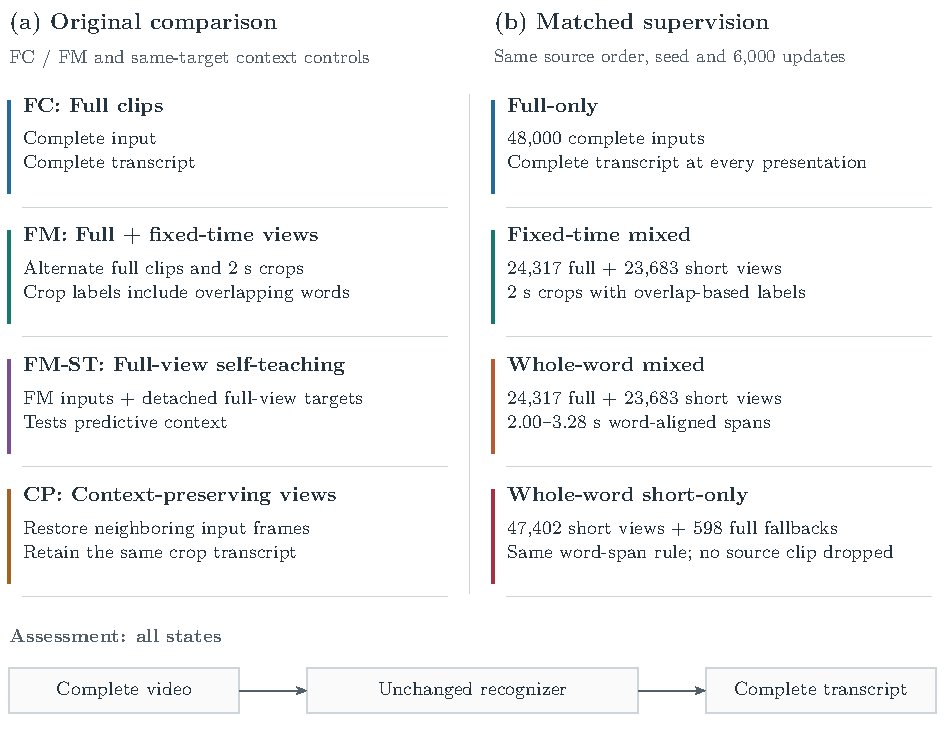
\includegraphics[width=\linewidth]{training_design.pdf}
 \caption{Training interventions with unchanged whole-utterance inference.
 (a) The original comparison tests full-clip continuation (FC), fragment mixing
 (FM), full-view self-teaching (FM-ST/T2), and restored visual context (CP/T4).
 (b) The matched comparison includes full-only, fixed-time mixed, whole-word
 mixed and whole-word short-only supervision. The mixed states share fallback
 positions; the short-only state also replaces the scheduled full views when
 an admissible word span exists. The two panels represent distinct fitted-state comparisons;
 all variants recognize the complete video at assessment. Schematic only.}
 \label{fig:design}
\end{figure}

\subsection{Conventional whole-word mixing}
\label{sec:wordviews}
To compare fragment labelling rules, we also construct short views containing
consecutive complete word annotations. For each scheduled fixed-time interval,
we enumerate annotation-bounded spans overlapping that interval, round their
start down and end up to frame indices, and retain lengths of 50--82 frames
(2.00--3.28 seconds). Among spans with nonempty, CTC-feasible labels, we choose
the one closest to the original interval's two boundaries. Ties are resolved
by proximity to 50 frames, midpoint distance and temporal order. The label
contains the consecutive words defining that span. Completeness refers to the
available annotations, not independently verified articulation boundaries.

This conventional alternative retains the alternating full/short schedule and
unchanged whole-utterance inference. When no admissible word span exists, both
the whole-word and fixed-time arms use the complete clip at that presentation.
Sharing these fallback positions prevents a difference in example coverage from
being mistaken for a crop effect. The comparison changes crop extent and target
content together; it does not hold input frames or target tokens exactly equal.

\subsection{Whole-word short-only supervision}
\label{sec:shortonly}
To test whether scheduled full-utterance supervision is needed alongside short
views, the short-only control preserves the whole-word mixed arm's source order
and all of its odd-indexed short views. At each formerly full, even-indexed
presentation, it applies the same deterministic fixed-time anchor and the
whole-word span rule in Section~\ref{sec:wordviews}. The target contains only the
words defining the selected span. When no admissible span exists, the complete
clip and transcript are retained; no source clip is removed or replaced.

This produces 47,402 short views and 598 full-clip fallbacks in 48,000
presentations. Of the fallbacks, 317 are the positions already shared by the two
mixed states and 281 occur at formerly full positions. Thus, ``short-only'' names
the intended supervision schedule, not the absence of every full-clip example.
The actual exposure is 2,719,321 input frames and 422,153 target tokens, with
470,153 valid attention positions including end-of-sequence tokens. The native
recognition objective, initializer, source order, optimizer schedule and final
6,000-update endpoint remain the same as in the matched mixed comparison.
This control changes the balance of full and short supervision; it does not
equalize frame exposure, target-token exposure or gradient magnitudes.

\subsection{Controlling loss reduction}
Short views change both the visual evidence and the number of supervised tokens.
We therefore compare native reduction with a paired, per-example normalized
objective. For a target of $N$ native tokens, the control minimizes
\begin{equation}
 \mathcal L_{\rm norm}(H,y)
 =0.1\frac{\mathcal L_{\ctc}^{\rm sum}(H,y)}{N}
 +0.9\frac{\mathcal L_{\att}^{\rm sum}(H,y)}{N+1}.
 \label{eq:normalized}
\end{equation}
The attention term retains the recognizer's native criterion; its denominator
counts valid target positions including the end-of-sequence token. The same
reduction applies to full and fragment presentations. This changes the weighting
of examples of different lengths and the relative contributions of the two
loss components. It does not match gradient norms or optimizer trajectories.
The comparison asks whether the full-versus-fragment transfer contrast persists
under this explicit reduction change.

\subsection{Controls for the role of context}
Two variants examine whether the information removed by cropping changes the
effect. Both retain the same full/fragment schedule, fragment labels, source clips
and final update count. They modify only the fragment presentations described
below. Their computational costs need not equal that of FM.

\paragraph{Full-view self-teaching (FM-ST; T2)}
The student processes $X_I$ as in FM. A second forward pass processes the complete
clip with the current model in evaluation mode and without gradients. Its encoded
features are restricted to $I$ before forming the teacher's CTC distribution.
Let $z_t^I$ be the student's CTC logits and $z_t^F$ the corresponding full-view
logits. With temperature $\tau=2$, the fragment objective is
\begin{align}
 p_t^F &= \sg\!\left[\operatorname{softmax}(z_t^F/\tau)\right],\\
 \mathcal L_{\rm FM\text{-}ST}
 &= \mathcal L_{\rm ASR}(f_\theta(X_I),y_I)
 + \lambda\frac{\tau^2}{L}
   \sum_{t=1}^{L}\KL\!\left(p_t^F\,\Vert\,
             \operatorname{softmax}(z_t^I/\tau)\right),
 \label{eq:teacher}
\end{align}
where $\lambda=0.15$. The teacher shares the current parameters with the student;
it is not an independently trained or exponential-moving-average model. Evaluation
mode removes training-mode stochasticity from the teacher pass. This control asks
whether a distribution informed by the complete video helps resolve the fragment's
reduced evidence. At test time the auxiliary pass and loss are absent.

\paragraph{Context-preserving continuation (CP; T4)}
The input to the encoder is expanded to $J=[a-16,b+16)$, retaining 0.64 seconds on
each side of the two-second fragment. Only the encoded positions corresponding to
$I$ are passed to the supervised recognition heads:
\begin{equation}
 \mathcal L_{\rm CP}
 =\mathcal L_{\rm ASR}\!\left(
          [f_\theta(X_J)]_{16:16+L},y_I\right).
 \label{eq:context}
\end{equation}
The target label and core pixels are identical to the corresponding FM
presentation. Neighboring pixels can affect the core representation through the
encoder, but neighboring words are not added to the supervised target merely
because context is visible. This separates retaining visual context from
restoring the complete transcript. It also differs from inference-time temporal
projection: no predicted word is selected by a timestamp at assessment.

\subsection{Comparison structure}
FC versus FM measures the net effect of replacing half the full presentations
with fragments. Whole-word mixing tests a conventional alternative to the
fixed-time label rule. Whole-word mixed versus short-only supervision tests
the contribution of scheduled full-utterance examples under the same short-view
rule. CP and FM-ST restore context through pixels and predictive
distributions, respectively, while keeping fragment targets fixed. Because an
overlap-selected label can extend beyond the crop, we report annotation coverage
alongside training exposure and complete-transcript recognition error.

\section{Experimental design}
\subsection{Corpora and recognition systems}
We evaluate the same continuation intervention in two corpus-transfer settings:
VLR to ViCocktail and LRS2 to WildVSR. Each setting has matched within-setting
FC/FM comparisons and two same-target context controls. Differences between
the corpus pairs include language, initialization, training coverage and
development-data availability; their comparison assesses portability rather
than isolating a single factor.

The Vietnamese setting continues a VLR recognizer on VLR training clips and
evaluates whole-utterance transfer to ViCocktail. VLR contains Vietnamese
mouth-video segments and associated text \cite{vlr2026dataset}; ViCocktail is a
separately constructed Vietnamese audiovisual corpus \cite{nguyen2025vicocktail}.
The assessment covers 1,167 official ViCocktail test clips, containing 30,091
whitespace-delimited reference units and 20 original-video groups. These groups
are recording-source identifiers, not verified speaker identities.

The English setting starts from an LRS3-initialized model, continues on prepared
LRS2 training clips, and evaluates all 2,854 released WildVSR clips, with 48,037
reference words \cite{afouras2022deep,afouras2018lrs3,djilali2024wildvsr}.
The source and destination terminology refers to continuation and assessment
corpora; the initializer can have its own upstream training history. We retain a
larger-data Auto-AVSR model as a practical English reference. It was trained with
LRS2, LRS3, VoxCeleb2 and AVSpeech, and is not an equal-resource continuation arm.

\begin{table}[tbp]
\centering\small
\caption{Data and exposure in the two continuation settings. Pool sizes refer to
the prepared inputs for this study, not the total size of the original datasets.}
\label{tab:data}
\begin{tabular}{lrr}
\toprule
Quantity & Vietnamese & English\\
\midrule
Prepared training clips & 92,632 & 45,838\\
Fragment-eligible training clips & 90,519 & 7,291\\
Distinct clips seen per matched run & 48,000 & 7,291\\
Training presentations per run & 48,000 & 48,000\\
Development clips for decoder selection & 768 & 1,082\\
Assessment clips & 1,167 & 2,854\\
Assessment reference units & 30,091 & 48,037\\
Seeds in completed FC/FM comparison & 17, 29 & 17\\
\bottomrule
\end{tabular}
\par\smallskip\begin{minipage}{\linewidth}\footnotesize
Vietnamese decoder selection uses ViCocktail development data; English selection
uses LRS2 source-development data. Vietnamese whitespace units and English words
are evaluated separately, without pooling their denominators.
\end{minipage}
\end{table}

Both continuation settings use the Auto-AVSR graph \cite{ma2023autoavsr}: a
3D convolution followed by a framewise ResNet-18, a 12-block Conformer encoder
with 768-dimensional representations, 12 attention heads and 3,072-dimensional
feed-forward layers, and a six-block Transformer decoder of the same width.
The Conformer convolution kernel has length 31. The Vietnamese initializer is
the VLR checkpoint; the English initializer is the released LRS3-trained
\texttt{vsr\_trlrs3\_base} checkpoint. Model identities and tokenizer mappings
are provided with the numerical supplement.

VLR supplies word timings in its annotation files. LRS2 main transcripts are
preserved, with missing word boundaries derived by audio CTC forced alignment.
Timings select training labels only; neither audio nor timings are supplied to
the visual recognizer at inference. Both sets of training timings are automatic.

Both settings use video alone at inference. The prepared grayscale mouth regions
have size $96\times96$; training center-crops them to $88\times88$ and normalizes
intensities with mean 0.421 and standard deviation 0.165 after scaling to $[0,1]$.
The continuation arms within a language share preprocessing, architecture and
tokenizer. The Vietnamese and English output inventories have 2,002 and 5,049
classes, respectively, including the required special symbols.
Figure~\ref{fig:datasets} illustrates the prepared mouth-region input in each
corpus, with source and destination roles defined by the transfer comparison.

\begin{figure}[tbp]
 \centering
 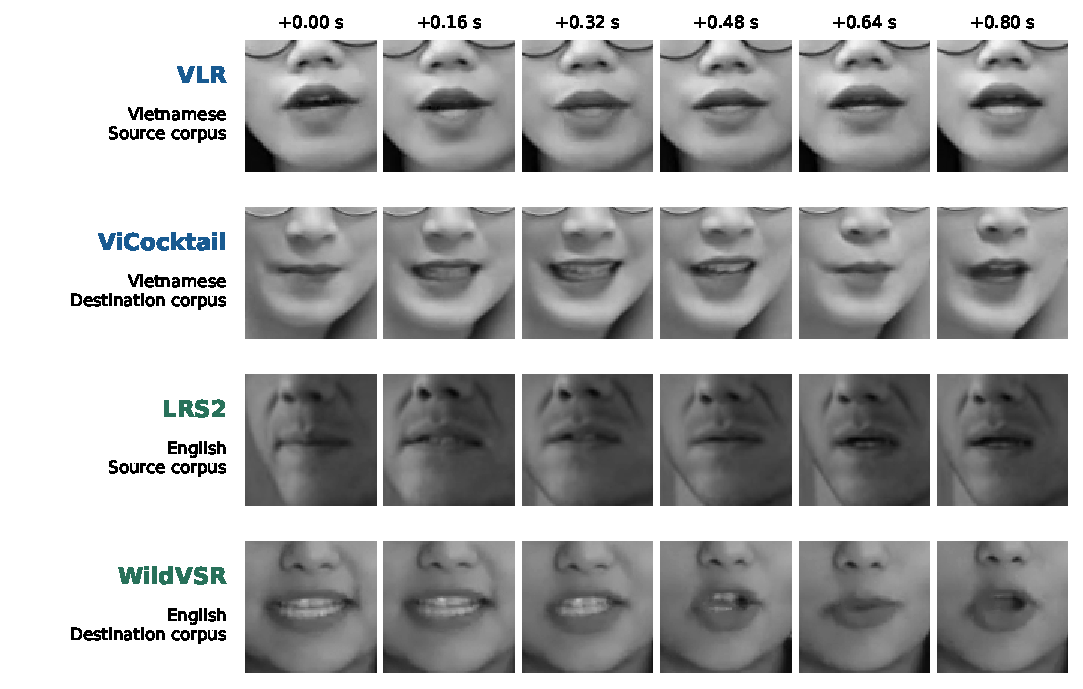
\includegraphics[width=\linewidth]{dataset_examples.pdf}
 \caption{Prepared mouth-region sequences from VLR~\cite{vlr2026dataset},
 ViCocktail~\cite{nguyen2025vicocktail}, LRS2~\cite{afouras2022deep} and
 WildVSR~\cite{djilali2024wildvsr}. Each row shows six real grayscale
 $88\times88$ center crops at 0.16-second intervals from one clip; displayed
 times are relative to the first illustrated frame. These examples show the
 visual input, while recognition is evaluated on complete clips.}
 \label{fig:datasets}
\end{figure}

A source-performance follow-up evaluates the initializer, FC and FM at seed 17
on all 11,307 prepared VLR test clips (225,960 reference units and 61 archived
source groups) and all 1,243 LRS2 test clips (6,660 words and 354 source groups).
Each corpus uses the same fitted states, preprocessing and frozen readouts as
its destination comparison. Source and destination results are analyzed
separately; the source follow-up does not add a second training seed.

\subsection{Continuation budget and controls}
All matched FC/FM comparisons use the final checkpoint after 6,000 updates, rather
than independently selected intermediate steps. The FM-ST and CP controls also
use step 6,000 and are evaluated at seed 17 in both corpus pairs. Training uses AdamW with peak
learning rate $2\times10^{-6}$, weight decay 0.01, 500 warm-up steps and cosine
decay. Eight individually processed examples are accumulated per optimizer step;
the gradient norm is clipped at 5. Training uses bfloat16 where supported, while
the assessment decoder uses float32. The same seed determines the source-clip
order and fragment choices across paired methods.

The fragment-eligibility rule requires 82--400 prepared frames, usable timing
and feasible target sequences. This has different consequences across corpora.
The Vietnamese matched runs draw 48,000 distinct clips from a pool of 90,519. The
English runs draw from 7,291 eligible clips, each revisited six or seven times.
Thus, both English FC and FM share the long-clip subset; FC does not receive the
short clips excluded from that matched comparison. An additional English full-pool
FC run (F0) uses the complete eligible full-clip pool of 45,838 clips at the same
6,000-update budget. It tests a practical alternative training population, rather
than isolating the crop transformation on identical examples.

We report the uncontinued initializer in each setting. We also report a native
ViCocktail model and the larger-data English Auto-AVSR model to indicate the
remaining performance gap. These practical references have different training
resources; the native ViCocktail system also has its own preprocessing. They are
not used to estimate the effect of FM relative to FC.

\subsection{Matched comparison of fragment labelling rules}
\label{sec:matchedcrop}
A follow-up VLR-to-ViCocktail experiment trains full-only, fixed-time and
whole-word continuations together in one training runtime at seed 17.
All three start from the same initializer and use the same 48,000 source-clip
presentations, 6,000 updates, optimizer schedule and native hybrid objective.
The two mixed arms share 317 full-clip fallback positions, yielding 24,317 full
and 23,683 short presentations per arm. They are newly fitted states, distinct
from the original FC/FM checkpoints. Their own source assessment covers all
11,307 VLR test clips under the same common decoder, with paired intervals
resampling the 61 source-video groups. Each new state is therefore assessed
on both source and destination without changing its weights or readout.

The crop rules in Section~\ref{sec:wordviews} and the final-update endpoint are
fixed before this follow-up's assessment. Its main comparison uses the common
decoder on the same 1,167 ViCocktail clips, without choosing a separate decoder
for each new model. This is a focused augmentation control on a previously used
assessment set, not a new independent corpus confirmation. Its conditional
intervals use the same 20 source groups and 10,000 paired resamples. We report
this comparison separately so that the shared fallbacks and fitted states are
not conflated with the original two-seed experiment.

A further pre-specified short-only state at seed 17 uses the schedule in
Section~\ref{sec:shortonly}; the three completed native states remain its fixed
comparators. Its assessment protocol covers the same 11,307 VLR source clips
and 1,167 ViCocktail destination clips, using the common decoder without a new
decoder search. The primary contrast is whole-word mixed minus short-only WER;
the reference contrast is full-only minus short-only WER. Positive differences
favor short-only supervision. Fixed-time mixing is a supporting comparison,
rather than an additional primary contrast. The two population-specific analyses
use 10,000 paired resamples of the 61 VLR or 20 ViCocktail archived source groups.
The plan and contrast directions were fixed before short-only training.
Intervals are conditional on these fitted states, pointwise and unadjusted for
multiplicity. No equivalence margin was specified, so an interval spanning zero
does not establish that mixing and short-only supervision are equivalent.
This follow-up also reuses previously observed assessment corpora and adds no
new training seed or independent test collection.

The loss-reduction control fits a further full-only/fixed-time pair using
Equation~\ref{eq:normalized}, with the same initializer, source schedules,
shared fallbacks, seed, optimizer and final-update endpoint as the matched crop
comparison. All four native/normalized states use the common decoder. We compute
the difference between their full-minus-fixed-time gains using paired resamples
of the same recording groups across all four states. No normalized whole-word
arm is included in this comparison.

\subsection{Decoder selection and metrics}
For the original FC/FM comparisons and same-target context controls, each
checkpoint's primary decoder is selected by aggregate error count on development
data from a fixed set of 11 candidates. The matched crop, short-only and
loss-reduction follow-ups use the common decoder without a new search. The candidates comprise hybrid
beam decoding with CTC weights $\alpha\in\{0.1,0.5,0.9,1.0\}$ and greedy CTC with
blank-logit biases $b\in\{0,-0.5,0.5,-1,1,-2,2\}$. Ties use a fixed candidate
order. Beam decoding uses width 40, zero length penalty and no external language
model. The search horizon covers the full encoded frame sequence. The common
decoder is the same beam decoder with $\alpha=0.1$ for all checkpoints.

Vietnamese primary selection uses 768 ViCocktail development clips, whereas
English selection uses 1,082 LRS2 source-development clips. Vietnamese therefore
allows target-domain decoder calibration without target-domain gradient updates;
English uses source-only decoder calibration. We do not treat these as identical
zero-shot protocols. The common-decoder comparison removes model-specific decoder
selection, although it cannot remove differences in the corpora or initializers.

Text is normalized with Unicode NFC, lowercasing and whitespace normalization.
We compute corpus-level WER as $100(S+D+I)/N$, where $N$ is the total reference
unit count. Vietnamese whitespace-delimited units need not coincide with lexical
words; consequently, its WER is not pooled with English WER. We report absolute
percentage-point differences and the underlying substitution, deletion and
insertion counts. Positive FC--FM differences favor FM.

Paired bootstrap intervals use 10,000 resamples. Vietnamese resampling preserves
the 20 original-video groups; WildVSR resampling uses released clips because a
validated recording-group reconstruction is unavailable. The WildVSR intervals are
therefore conditional clip-resampling summaries and do not establish uncertainty
over independent recording sources. The source follow-up resamples 61 VLR or
354 LRS2 archived source groups, which are not asserted to be verified speaker
identities. These resampling units differ across corpora. All intervals condition on the
fitted seeds and chosen decoders. For the mechanism comparison, FM--FM-ST and
FM--CP are the primary contrasts; comparisons with FC describe how much of the
original transfer gain remains. Intervals are pointwise, without adjustment for
multiple comparisons. The assessment sets have appeared in earlier
experiments; the results should therefore be interpreted as retrospective
evidence rather than confirmation on an untouched test set. The source-performance follow-up also uses previously observed test data.
Upstream training overlap is not independently established.

\section{Results}
\subsection{Transfer under a common decoding rule}
The two corpus pairs produce different outcomes under the same within-setting
comparison. FM improves VLR-to-ViCocktail transfer by 3.410 and 3.170 WER points
at seeds 17 and 29. It produces no clear LRS2-to-WildVSR improvement: the
common-decoder FC--FM difference is $-0.067$ points, with an interval that
includes zero. Figure~\ref{fig:gains} and Table~\ref{tab:comparisons} summarize
these contrasts. We first examine destination transfer and the corresponding
source assessment, then analyze error changes, training exposure and contextual
information.

\subsubsection{VLR to ViCocktail}

Table~\ref{tab:vi} presents the VLR-to-ViCocktail comparison. With the common
beam decoder, replacing half the full-clip presentations with fragments reduces
WER from 67.326 to 63.916 at seed 17 and from 67.233 to 64.062 at seed 29.
The gains of 3.410 and 3.170 percentage points therefore persist with the same
recognizer architecture, source-clip schedule, update count and decoding rule.
They measure the benefit of the training intervention under this continuation
budget, rather than a benefit from model-specific decoder selection.

\begin{table}[tbp]
\centering\small
\caption{Whole-utterance transfer from VLR to ViCocktail. WER (\%) is lower when better.}
\label{tab:vi}
\begin{tabular}{llrrl}
\toprule
Model & Seed & Primary & Common & Primary decoder \\
\midrule
Initial & -- & 70.057 & 70.034 & Greedy $b=-1$ \\
FC & 17 & 67.445 & 67.326 & Greedy $b=-1$ \\
FM & 17 & 61.882 & 63.916 & $\alpha=0.5$ \\
FM-ST & 17 & 62.002 & 63.919 & $\alpha=0.9$ \\
CP & 17 & 62.444 & 64.793 & $\alpha=0.5$ \\
FC & 29 & 66.983 & 67.233 & Greedy $b=-1$ \\
FM & 29 & 63.448 & 64.062 & Greedy $b=-1$ \\
Native ViCocktail & -- & 38.503 & 38.503 & $\alpha=0.1$ \\
\bottomrule
\end{tabular}
\par\smallskip\begin{minipage}{\linewidth}\footnotesize Primary decoders use 768 ViCocktail development clips. The common decoder has CTC weight 0.1 and beam size 40. FM-ST and CP have seed 17 only. The native reference uses different training data and preprocessing.
\end{minipage}
\end{table}


Development-selected decoding strengthens the seed-17 result: FC/FM obtain
67.445/61.882 WER, a 5.563-point gain. At seed 29, the corresponding values are
66.983/63.448, a 3.536-point gain. The interaction with decoding affects the
magnitude, but not the direction, of the Vietnamese result. FM also improves on
the uncontinued initializer, which obtains 70.057 primary and 70.034 common-decoder
WER. The native ViCocktail reference reaches 38.503 WER with different training
resources and preprocessing. FM thus improves cross-corpus continuation while
leaving a substantial gap to a system developed for the destination corpus.

Both seeds improve in all 20 original-video groups under either decoding regime.
The common-decoder source-bootstrap 95\% intervals are [2.892, 4.119] and
[2.683, 3.885] points (Table~\ref{tab:comparisons}; Figure~\ref{fig:gains}).
This consistency supports a gain within the studied corpus pair. The intervals
summarize variation across observed recording groups conditional on the fitted
models; they do not estimate variability across independently trained seeds.

\begin{table}[tbp]
\centering\small
\caption{Paired FC--FM improvements and 95\% bootstrap intervals (percentage points).}
\label{tab:comparisons}
\begin{tabular}{llrrr}
\toprule
Transfer & Seed & Regime & Gain & 95\% interval \\
\midrule
VI & 17 & Primary & 5.563 & [4.940, 6.351] \\
VI & 29 & Primary & 3.536 & [2.360, 4.768] \\
VI & 17 & Common & 3.410 & [2.892, 4.119] \\
VI & 29 & Common & 3.170 & [2.683, 3.885] \\
EN & 17 & Primary & 0.025 & [-0.371, 0.428] \\
EN & 17 & Common & -0.067 & [-0.338, 0.210] \\
\bottomrule
\end{tabular}
\par\smallskip\begin{minipage}{\linewidth}\footnotesize Positive values favor FM. Vietnamese intervals resample original-video groups; English intervals resample released clips. Intervals condition on the fitted models and decoders.
\end{minipage}
\end{table}


\begin{figure}[tbp]
 \centering
 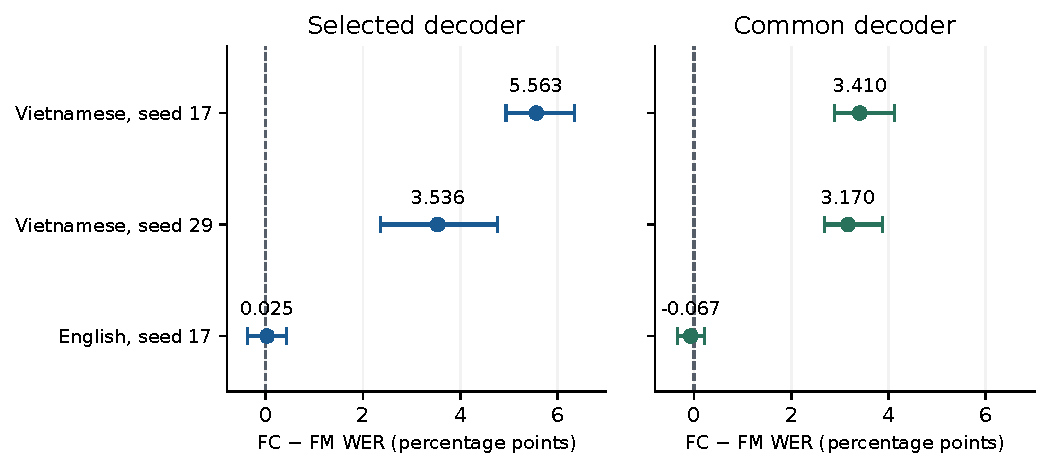
\includegraphics[width=\linewidth]{paired_gains.pdf}
 \caption{Paired FC--FM gains in whole-utterance WER. Positive values favor FM.
 Error bars are 95\% bootstrap intervals. Vietnamese intervals resample original
 videos; English intervals resample released clips. The English result provides
 a cross-setting check, without pooling the two languages.}
 \label{fig:gains}
\end{figure}

\subsubsection{LRS2 to WildVSR}

The English experiment checks the same recipe in a different continuation
setting. It does not reproduce the Vietnamese advantage (Table~\ref{tab:en}).
Primary FC/FM WER is 66.817/66.792: a 0.025-point gain with a conditional
clip-bootstrap interval of [$-0.371$, 0.428]. Under the common decoder, FM is
slightly worse, 66.884 versus 66.817, with an FC--FM interval of
[$-0.338$, 0.210]. The initializer obtains 66.164 primary and 67.092 common WER.
FM is therefore descriptively worse than the initializer under selected decoding,
but slightly better under common decoding; continuation is not uniformly helpful.

\begin{table}[tbp]
\centering\small
\caption{Whole-utterance transfer to WildVSR. WER (\%) on the same 2,854 assessment clips.}
\label{tab:en}
\begin{tabular}{llrrl}
\toprule
Model & Seed & Primary & Common & Primary decoder \\
\midrule
Initial & -- & 66.164 & 67.092 & $\alpha=0.5$ \\
FC & 17 & 66.817 & 66.817 & $\alpha=0.1$ \\
FM & 17 & 66.792 & 66.884 & $\alpha=0.5$ \\
FM-ST & 17 & 66.771 & 66.894 & $\alpha=0.5$ \\
CP & 17 & 66.749 & 66.794 & $\alpha=0.5$ \\
Full-pool FC & 17 & 67.438 & 67.438 & $\alpha=0.1$ \\
Large-data Auto-AVSR & -- & 36.010 & 36.010 & $\alpha=0.1$ \\
\bottomrule
\end{tabular}
\par\smallskip\begin{minipage}{\linewidth}\footnotesize Primary decoders use 1,082 LRS2 source-development clips. The common decoder has CTC weight 0.1 and beam size 40. All continuation variants use seed 17. Full-pool FC changes the training population; the large-data reference uses different pretraining resources.
\end{minipage}
\end{table}


The training regimes differ materially. English fragment eligibility retains
7,291 of 45,838 prepared clips (15.91\%), increasing mean training duration from
2.183 to 4.404 seconds. Each eligible clip is presented six or seven times,
whereas each selected Vietnamese clip appears once. Using the complete English
pool in the equal-step F0 control gives 67.438 WER, worse than matched-pool FC
by 0.620 points (95\% interval [0.298, 0.950]). This alternative does not recover
the gain; it changes content, duration and repetition together, and cannot show
that additional data is intrinsically harmful.

The assessment durations are more similar: Vietnamese mean/median length is
145.74/129 frames, versus 151.31/139 in English. English's largest length stratum
is nearly tied and the stratum above 200 frames is slightly worse with FM.
The contrast therefore cannot be explained simply by shorter English test clips.
The larger-data English reference reaches 36.010 WER, emphasizing the remaining
gap to stronger training resources. Taken together, the English results bound
the portability of FM and motivate studying exposure and supervision conditions,
rather than attributing the difference to language alone.

\subsection{Does the gain require fixed-time boundary supervision?}
\label{sec:cropresults}
The matched augmentation follow-up directly compares fixed-time fragments with
conventional whole-word views (Section~\ref{sec:matchedcrop}). Table~\ref{tab:crop}
shows the four matched states under the common decoder. We first compare the
three crop-control states. Fixed-time mixing
reduces WER from 67.369 to 63.846, a 3.523-point gain with a conditional
95\% group-bootstrap interval of [2.985, 4.179]. Whole-word mixing reaches
63.388 WER, improving over full-only by 3.981 points \mbox{[3.420, 4.731]}.

\begin{table}[tbp]
\centering\small
\setlength{\tabcolsep}{4pt}
\caption{Source and destination performance of the matched continuation recipes
at seed 17. The same fitted states use a common decoder on 11,307 VLR and
1,167 ViCocktail clips. Training frame and native-token counts are in millions.}
\label{tab:crop}
\begin{tabular}{lrrrr}
\toprule
Training views & VLR WER (\%) & ViCocktail WER (\%) & Frames & Tokens\\
\midrule
Full-only & 38.029 & 67.369 & 7.307 & 1.145\\
Fixed-time mixed & 38.580 & 63.846 & 4.888 & 0.798\\
Whole-word mixed & 38.606 & 63.388 & 5.013 & 0.784\\
Whole-word short-only & 44.844 & 70.715 & 2.719 & 0.422\\
\bottomrule
\end{tabular}
\par\smallskip\begin{minipage}{\linewidth}\footnotesize
Each arm uses 48,000 source presentations and 6,000 updates. Both mixed arms
share 317 full-clip fallbacks; short-only uses 598 fallbacks (1.25\%).
These fitted states are distinct from the original FC/FM comparison.
Frame and token exposures are not equal.
\end{minipage}
\end{table}


Whole-word mixing is better than fixed-time mixing by 0.459 points
[0.268, 0.674]. Its 138 fewer errors comprise 106 fewer deletions and 78 fewer
insertions, offset by 46 additional substitutions. The transfer benefit thus
persists with conventional word-aligned views, and the tested fixed-time rule
does not provide an additional advantage over the tested whole-word alternative
under this protocol. This supports mixed short supervision
as a useful continuation choice here without requiring incomplete boundary
evidence as its explanation.

The same three fitted states also expose the source cost of these transfer
gains. On all 11,307 VLR test clips, WER is 38.029 for full-only, 38.580 for
fixed-time and 38.606 for whole-word continuation. Relative to full-only,
the source costs are 0.551 points [0.439, 0.664] for fixed-time and
0.577 points [0.448, 0.705] for whole-word mixing. Both arise primarily from
more deletions, despite fewer substitutions. Whole-word source WER exceeds
fixed-time WER by 0.026 points, with an interval of [$-0.043$, 0.091].
This comparison does not resolve a source-performance difference between the
two crop rules or establish their equivalence. Whole-word mixing delivers the
larger measured destination gain; neither mixed recipe improves uniformly
over full-only continuation across source and destination.

The three crop-control arms receive the same source presentations and updates. Whole-word
mixing nevertheless processes 2.55\% more frames and 1.70\% fewer target tokens
than fixed-time mixing. The comparison therefore evaluates two practical crop
recipes rather than isolating a single boundary variable. It is a one-seed
follow-up on the previously used assessment corpus, with shared fallback
positions. The original FM source/destination profile below belongs to different
fitted states; Table~\ref{tab:crop} reports the new controls' own source assessment.

\subsection{Does the gain persist without scheduled full-clip supervision?}
\label{sec:shortonlyresults}
The short-only state obtains 70.715\% ViCocktail WER and 44.844\% VLR WER
(Table~\ref{tab:crop}). The predeclared whole-word mixed--short-only differences
are $-7.328$ destination points [${-8.864}$, ${-5.488}$] and $-6.238$ source
points [${-6.592}$, ${-5.887}$], favoring mixing in both populations.
Short-only is also worse than full-only continuation by 3.347 destination
points and 6.815 source points (Table~\ref{tab:shortonly}).

\begin{table}[tbp]
\centering\small
\caption{Predeclared comparisons with whole-word short-only continuation.
Differences are reference minus short-only WER in percentage points;
positive values favor short-only. Mixed denotes whole-word mixing.}
\label{tab:shortonly}
\begin{tabular}{llrr}
\toprule
Population & Contrast & Difference & 95\% interval\\
\midrule
VLR & Mixed--short-only & -6.238 & [-6.592, -5.887]\\
VLR & Full--short-only & -6.815 & [-7.207, -6.440]\\
ViCocktail & Mixed--short-only & -7.328 & [-8.864, -5.488]\\
ViCocktail & Full--short-only & -3.347 & [-4.773, -1.341]\\
\bottomrule
\end{tabular}
\par\smallskip\begin{minipage}{\linewidth}\footnotesize
Pointwise intervals use 10,000 paired bootstrap resamples of 61 archived
VLR source groups or 20 ViCocktail recording groups, conditional on the fitted
states. Whole-word mixed versus short-only is the primary contrast;
full-only versus short-only is the reference contrast.
\end{minipage}
\end{table}


The loss is dominated by deletions. Relative to whole-word mixing, short-only
adds 5,735 deletions on ViCocktail; 3,098 fewer substitutions and 432 fewer
insertions leave 2,205 additional errors. On VLR, 33,541 additional deletions
outweigh 15,373 fewer substitutions and 4,072 fewer insertions, adding 14,096
errors. This error balance is consistent with poorer complete-transcript coverage,
but does not identify its internal cause.

Retaining scheduled full-utterance presentations therefore improves the tested
whole-word recipe at the same update budget. The benefit of mixing over full-only
continuation cannot be extended to a nearly all-short schedule: the latter uses
47,402 short views and 598 full fallbacks, and performs worse than both controls.
Frame and target-token exposure also decrease, so this comparison does not
isolate context length from objective exposure or establish an optimal mixing ratio.

\subsection{Does the transfer gain persist under token-normalized loss?}
\label{sec:lossresults}
The paired reduction control tests whether the fixed-time gain depends on
retaining the native unnormalized components. Table~\ref{tab:reduction} reports
the complete four-state comparison. With token-normalized loss, full-only and
fixed-time mixing obtain 67.223 and 63.763 WER. The gain is 3.460 points,
with a conditional 95\% recording-group interval of [2.756, 4.423].

\begin{table}[tbp]
\centering\small
\caption{Loss-reduction control on the complete ViCocktail assessment at seed 17.
All four fitted states use the common decoder. Gain is full-only minus fixed-time WER.}
\label{tab:reduction}
\begin{tabular}{lrrr}
\toprule
Loss reduction & Full-only WER & Fixed-time WER & Gain (pp)\\
\midrule
Native & 67.369 & 63.846 & 3.523\\
Token-normalized & 67.223 & 63.763 & 3.460\\
\bottomrule
\end{tabular}
\end{table}


The normalized-minus-native change in the gain is $-0.063$ points, with a
paired interval of [$-0.366$, 0.386]. Thus the transfer advantage remains under
the tested component-wise normalization. The interval does not establish exact
equivalence between reductions, but the result does not support an explanation
in which the gain disappears after dividing by target length. This one-seed
control strengthens the short-view finding under a second objective reduction;
it does not identify a unique optimization mechanism or predict how normalized
whole-word mixing would behave.

\subsection{Source and destination performance at the same fitted states}
\label{sec:source}
For the original continuation comparison, we assess the initializer, FC and FM
on the complete prepared source test sets:
11,307 VLR clips and 1,243 LRS2 clips. This retrospective follow-up uses the
same seed-17 checkpoints and readouts as the destination comparison, without
source-test decoder tuning. Table~\ref{tab:source} and Figure~\ref{fig:source}
show the resulting source/destination profiles.

\begin{table}[tbp]
\centering\small
\caption{Source and destination WER (\%) at the same fitted states and
common decoder. Source populations are 1,243 LRS2 clips (6,660 words)
and 11,307 VLR clips (225,960 whitespace units). Destination populations
are 2,854 WildVSR and 1,167 ViCocktail clips. Continuation results use seed 17;
each corpus is scored separately. Lower WER is better.}
\label{tab:source}
\begin{tabular}{lrrrr}
\toprule
& \multicolumn{2}{c}{English} & \multicolumn{2}{c}{Vietnamese}\\
\cmidrule(lr){2-3}\cmidrule(lr){4-5}
State & LRS2 & WildVSR & VLR & ViCocktail\\
\midrule
Initializer & 56.577 & 67.092 & 39.830 & 70.034\\
FC & 50.976 & 66.817 & 38.016 & 67.326\\
FM & 52.432 & 66.884 & 38.604 & 63.916\\
\bottomrule
\end{tabular}
\end{table}


On VLR, common-decoder WER is 39.830 for the initializer, 38.016 for FC and
38.604 for FM. The paired FC--FM difference is $-0.588$ points, with a
95\% source-group bootstrap interval of [$-0.709$, $-0.474$]. FM therefore
trades a modest source disadvantage relative to FC for its 3.410-point
ViCocktail improvement at this seed. It adds 1,329 source errors: 3,641
additional deletions outweigh 2,163 fewer substitutions and 149 fewer
insertions. Both continuations still improve on the initializer.

On LRS2, common-decoder WER is 56.577, 50.976 and 52.432 for the initializer,
FC and FM. FM produces 97 more errors than FC: 32 substitutions, 26 deletions
and 39 insertions across 6,660 reference words. The FC--FM difference is
$-1.456$ points, with an interval of [$-2.375$, $-0.584$]. Unlike the
Vietnamese profile, this source disadvantage has no demonstrated destination
benefit on WildVSR. It is a disadvantage relative to FC, not forgetting
relative to the initializer; the experiment does not measure the English
initializer's upstream LRS3 performance.

Decoder selection changes the Vietnamese source ranking. Applying the frozen
ViCocktail-development choices to VLR gives FC/FM WERs of 43.371/38.939 and
an FC--FM difference of 4.432 points [4.199, 4.658]. FC uses greedy CTC with
blank bias $-1$, whereas FM uses hybrid beam decoding with CTC weight 0.5.
These are destination-calibrated readouts, not source-optimal decoders, and
their contrast combines changes in the fitted model and decoding. The common
decoder exposes the smaller source cost described above. The English source
ranking is unchanged by its development-selected readouts: FC/FM WER is
50.976/52.883, a difference of $-1.907$ points [$-2.986$, $-0.831$].

\begin{figure}[tbp]
 \centering
 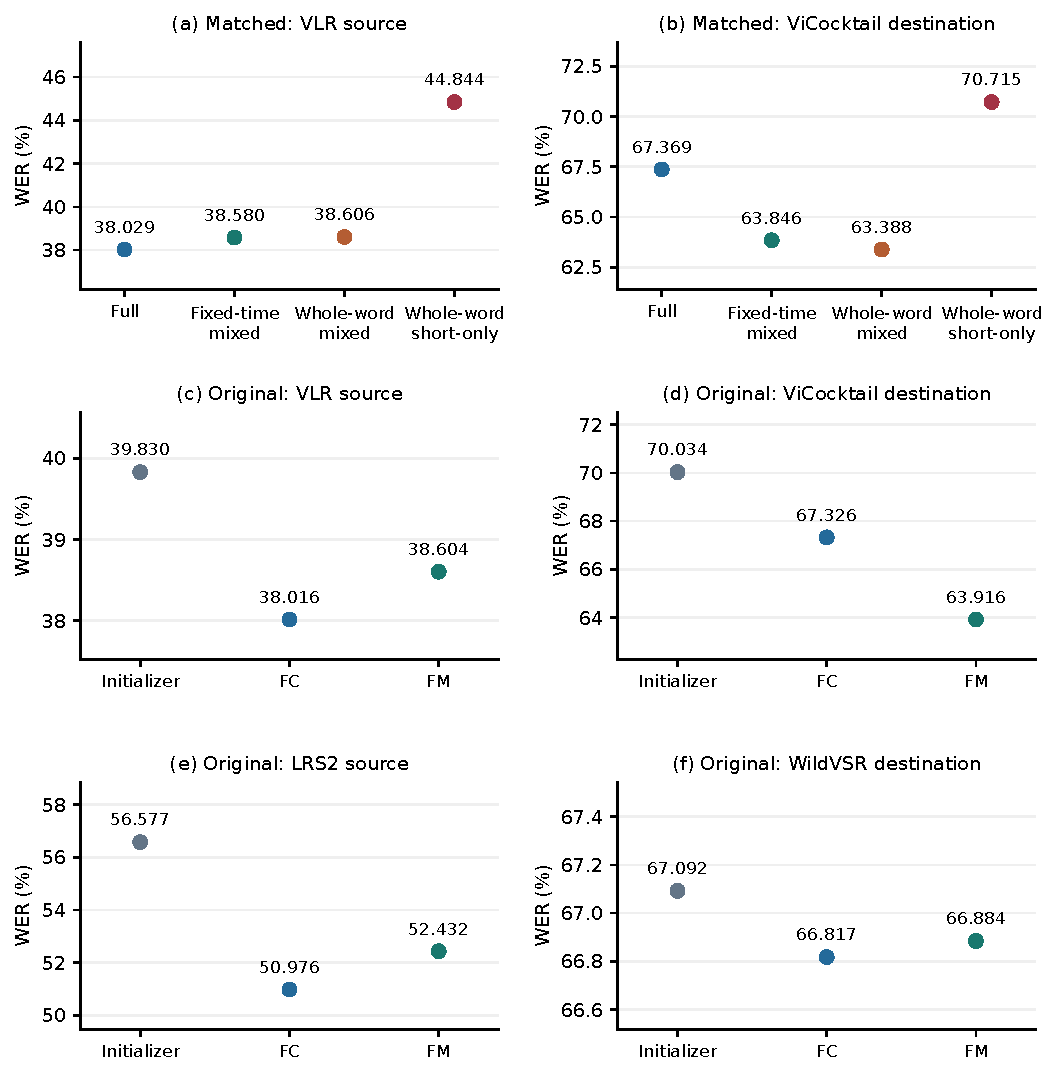
\includegraphics[width=\linewidth]{source_destination_profile.pdf}
 \caption{Source/destination WER at the same fitted seed-17 states under common
 decoding. (a,b) The matched full-only, fixed-time mixed, whole-word mixed and
 short-only states. (c,d) The original Vietnamese initializer/FC/FM comparison.
 (e,f) The original English comparison. Original and matched FC/FM states are
 distinct. Each panel has a separately labelled vertical scale; WERs are not
 averaged across corpora.}
 \label{fig:source}
\end{figure}

The source follow-up separates a transfer benefit from uniform improvement
across corpora. It also shows why source retention must be reported with its
readout: a ranking obtained with destination-calibrated decoders need not
match the ranking under shared decoding. Neither profile identifies the
learning mechanism responsible for the difference between continuation settings.

\subsection{Error changes and utterance length}
Under the common decoder, Vietnamese FM removes 1,026 errors at seed 17:
34 substitutions, 492 deletions and 500 insertions. At seed 29, it removes
954 errors: 35 substitutions, 371 deletions and 548 insertions
(Figure~\ref{fig:errors}). Most of the gain therefore comes from producing a
more accurate number of transcript units, rather than substituting fewer units.
The counts are consistent with a change in omission--insertion behavior; they
do not identify whether the cause lies in visual representations, attention
or confidence calibration.

\begin{figure}[tbp]
 \centering
 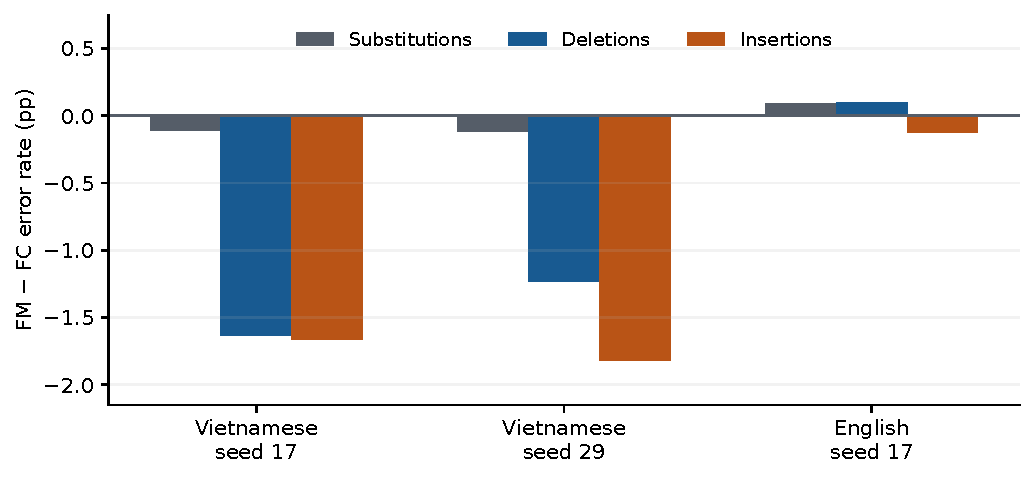
\includegraphics[width=\linewidth]{edit_changes.pdf}
 \caption{Common-decoder changes in substitution, deletion and insertion rates,
 computed as $100(\text{FM count}-\text{FC count})/N$. Negative values indicate
 fewer errors. Each setting uses its own complete assessment reference count.}
 \label{fig:errors}
\end{figure}

A post-hoc length analysis shows that the Vietnamese gain extends beyond short
utterances. The largest stratum, 101--200 prepared frames, contains 772 clips and
17,820 reference units. FM removes 398 and 349 errors at seeds 17 and 29,
respectively, reducing WER by 2.233 and 1.958 points. Clips above 200 frames also
improve, by 3.814 and 3.275 points. The 11 shortest clips contain only 57 reference
units and account for 58 and 63 errors removed; their extreme percentage-point
changes do not characterize the aggregate result. These descriptive strata were
formed after inspecting the aggregate outcomes.

\subsection{Training exposure and the role of context}
\label{sec:exposure}
FM changes the length of both the visual input and its supervision.
Table~\ref{tab:exposure} quantifies this change at the common final update.
Vietnamese FM uses approximately 66.4\% of FC's input frames and 69.1\% of its
target tokens in both seeds. Equal numbers of updates and presentations therefore
do not imply equal information exposure. These counts do not measure FLOPs,
runtime or gradient scale.

\begin{table}[tbp]
\centering\small
\caption{Training exposure at 6,000 updates. Every run has 48,000 presentations;
frame and native-token counts are shown in millions.}
\label{tab:exposure}
\begin{tabular}{llrrrr}
\toprule
Setting & Seed & FC frames & FM frames & FC tokens & FM tokens\\
\midrule
Vietnamese & 17 & 7.307 & 4.851 & 1.145 & 0.791\\
Vietnamese & 29 & 7.293 & 4.842 & 1.144 & 0.790\\
English & 17 & 5.284 & 3.843 & 0.831 & 0.629\\
\bottomrule
\end{tabular}
\end{table}

The two context controls retain FM's fragment targets. CP supplies neighboring
pixels, adding 768,000 encoder input frames across 24,000 fragment presentations.
FM-ST instead supplies a full-view predictive distribution through 24,000
additional teacher passes. At seed 17, total encoder input is 76.90\% of FC for
Vietnamese CP and 116.42\% for FM-ST (Figure~\ref{fig:contextbudget}). Teacher
passes do not backpropagate, so the ratios are exposure comparisons rather than
compute-matched budgets.

\begin{figure}[tbp]
 \centering
 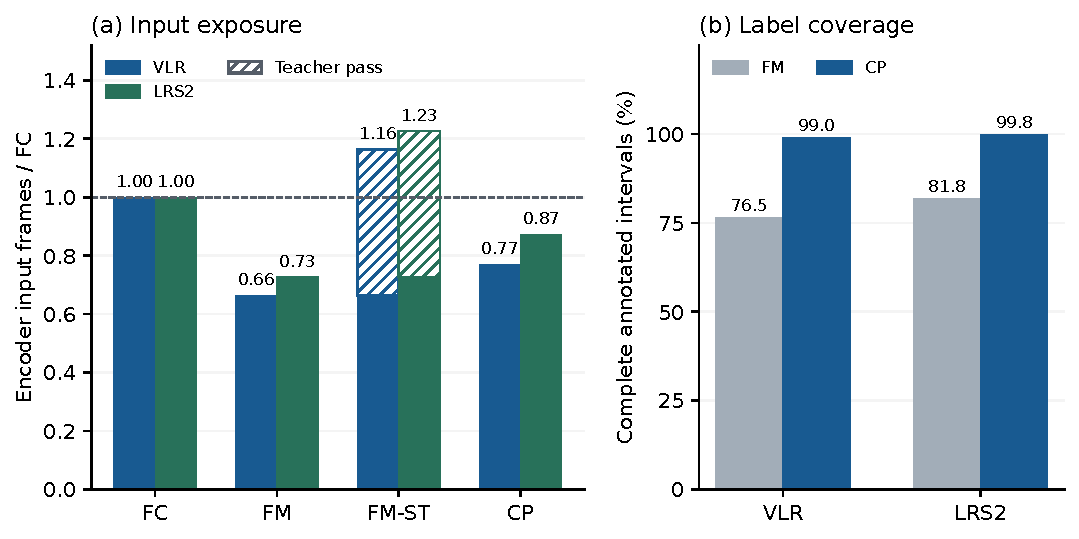
\includegraphics[width=\linewidth]{training_context_budget.pdf}
 \caption{Training-design measurements at seed 17. (a) Encoder input frames
 relative to FC, including the no-gradient teacher pass in FM-ST. (b) Selected
 positive-duration annotation intervals fully contained in the encoder input.
 Coverage uses all 24,000 fragment presentations per corpus and automatic
 timestamps; zero-duration entries are excluded.}
 \label{fig:contextbudget}
\end{figure}

Added context also restores visual evidence for labels touching a crop boundary.
The fraction of selected positive-duration annotation intervals fully contained
in the input rises from 76.49\% to 99.02\% in VLR, and from 81.79\% to 99.77\%
in LRS2. A one-frame tolerance preserves this contrast. The 2,378 zero-duration
VLR entries are excluded from coverage calculations but remain in training.
Thus, CP changes neighboring information and boundary-label coverage together;
it is not a pure intervention on context independent of label completeness.
Automatic timings describe annotation coverage, not verified visual articulation.

Neither control strengthens the main Vietnamese result. FM-ST reaches 62.002
primary and 63.919 common-decoder WER, compared with FM's 61.882 and 63.916.
The common-decoder difference is one error across 30,091 reference units; both
paired intervals include zero. The tested self-teaching loss therefore adds no
clear benefit at its specified temperature and weight.

CP reaches 62.444 primary and 64.793 common-decoder WER. It remains better than
FC by 5.001 and 2.532 points, but FM outperforms CP by 0.562 points under the
primary decoder (95\% interval [0.340, 0.826]) and 0.877 points under the common
decoder ([0.348, 1.422]). FM and CP select the same primary decoder.
Restoring most boundary-label coverage preserves a substantial benefit over FC,
while failing to improve FM. This supports further investigation of shorter
supervision; it does not establish that missing context causes the gain.

\begin{figure}[tbp]
 \centering
 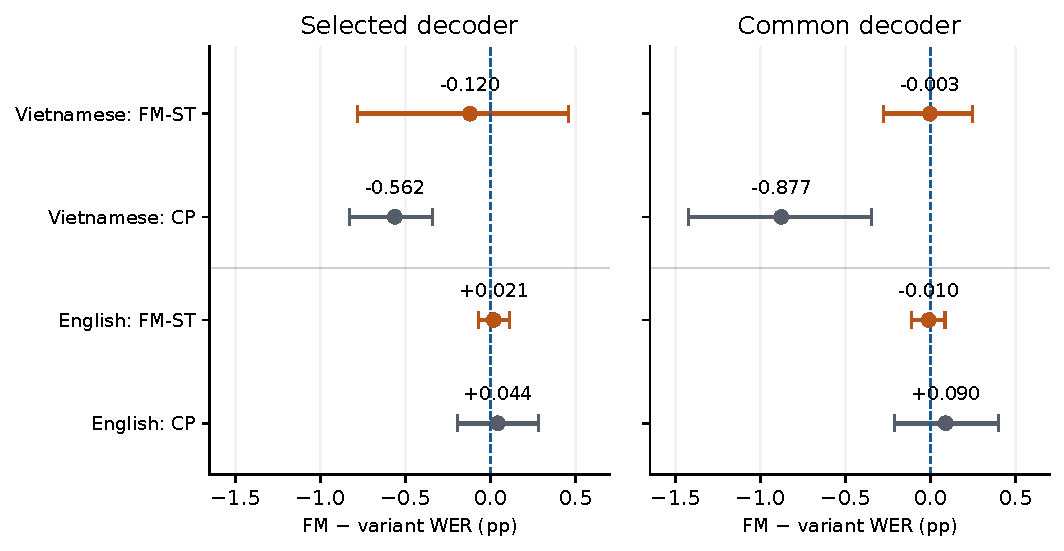
\includegraphics[width=\linewidth]{mechanism_gains.pdf}
 \caption{Paired effects of full-view self-teaching (FM-ST) and context
 preservation (CP) relative to FM at seed 17. Positive values favor the variant.
 Error bars are pointwise 95\% bootstrap intervals, conditional on fitted models
 and decoders, without multiple-comparison adjustment. Vietnamese resampling
 uses original-video groups; English resampling uses released clips.}
 \label{fig:mechanisms}
\end{figure}

CP's Vietnamese error balance differs from FM: 325 fewer substitutions and six
fewer insertions are offset by 595 additional deletions, producing 264 more
errors overall. This post-hoc decomposition shows why restoring visual coverage
or reducing one edit type need not improve complete-transcript WER.


In the English setting, FM-ST and CP remain near FM: their primary WERs are 66.771 and 66.749,
respectively, and all English FM--variant intervals include zero. Under the
common decoder, CP removes 621 substitutions and 461 insertions relative to FM
but adds 1,039 deletions, leaving only 43 fewer errors (0.090 points).
Likewise, common-decoder FM removes 59 insertions relative to FC but adds
44 substitutions and 47 deletions. The Vietnamese improvement in both insertion
and deletion counts does not carry over to this English setting.



\section{Discussion}
\subsection{When fragment supervision is useful}
The original Vietnamese FC/FM gain repeats across both fitted seeds and all
20 observed recording groups, mainly through fewer deletions and insertions.
It accompanies a source disadvantage relative to FC, while FM remains better
than the VLR initializer. English FM also retains less source improvement
than FC but gives no clear WildVSR benefit. These outcomes support a useful
continuation option in one regime, with different source/destination trade-offs.
Conventional whole-word mixing strengthens the Vietnamese transfer gain without
resolving its source cost. The effect therefore does not require incomplete
boundary evidence from fixed-time crops.

The short-only control makes the role of scheduled full supervision more concrete.
Replacing full views with additional whole-word fragments loses 7.328 destination
and 6.238 source WER points relative to whole-word mixing, with more deletions
outweighing fewer substitutions and insertions. An exploratory fixed greedy-CTC check retains the short-only disadvantage
against both full-only and whole-word mixed states on
both complete populations (Supplementary Material). This ordering is therefore
not confined to the common hybrid decoder, although the check
reuses the fitted states and assessment data. Retaining full presentations
helps under this update budget; mixing still incurs a source cost relative to
full-only. The comparison establishes neither an optimal ratio nor a universal
failure of short-only objectives or a single internal mechanism.

This distinction matters when selecting a continuation strategy. Source
recognition and destination recognition answer different questions, and their
WERs should be considered separately. Improving over the initializer on the
continuation source is insufficient to establish a destination benefit. Source
retention also depends on the readout: the Vietnamese FC/FM ranking reverses
when destination-calibrated decoders replace the shared decoder. Reporting both
comparisons distinguishes the fitted-state comparison from the deployed
model-plus-decoder choice, without treating either as a source-tuned optimum.

FM has a practical advantage in deployment complexity: it retains the same
single whole-utterance recognition procedure. It is relevant when source videos
and an existing recognizer are available but additional inference modules or
destination-domain gradient updates are undesirable. The Vietnamese experiment
does use destination development data for decoder calibration; the shared-decoder
result separates the observed gain from model-specific calibration. With the
remaining error rates, assisted transcription with human correction is a
plausible use case, rather than unattended transcription requiring high accuracy.
The application is a motivation; user-level utility has not been measured.

\subsection{What changes when context is restored}
The context-preserving control retains the fragment targets while restoring
neighboring visual evidence. It covers almost all selected annotation intervals
and retains part of the Vietnamese gain over FC, but performs worse than FM.
Its reduction in substitutions is outweighed by additional deletions. This
same-target contrast shows that more visible context is not sufficient to
improve the tested continuation recipe. It does not prove that deliberately
incomplete boundary evidence is the cause of the gain: context and label
coverage change together.

Full-view self-teaching provides contextual information through a predictive
distribution instead of additional student input. At the tested temperature and
weight, it adds no clear benefit. The additional context mechanisms therefore
have no demonstrated advantage over FM in these tests. Neither result establishes that all
forms of context restoration or distillation are ineffective.

FM couples shorter inputs, shorter supervision and native loss reduction.
The English setting also repeatedly revisits a smaller, length-selected source
pool, whereas the Vietnamese setting presents each selected source clip once.
These differences suggest that supervision exposure and continuation regime
deserve attention before attributing the contrast to linguistic structure.
The observed frame/token counts cannot determine gradient contributions or
compute efficiency. The completed whole-word comparison shows that the direction
of the transfer benefit can be obtained by conventional short-view augmentation;
it provides no evidence for a unique advantage of overlap-labelled boundaries.
Because crop lengths and target exposure still differ, its whole-word advantage
cannot be assigned solely to label completeness. The paired reduction control
retains a 3.460-point fixed-time gain after normalizing each loss component by
its valid target length, close to the native 3.523-point gain. This rules out
the simple claim that the observed advantage disappears under this reduction
change. It does not establish invariance to every objective scaling, and the
four loss-control states do not isolate a single causal optimization mechanism.

\subsection{Scope and reproducibility}
The evidence concerns two corpus pairs within one recognizer family. The
Vietnamese FC/FM comparison includes two seeds; the English comparison,
context controls and matched crop, short-only and loss controls use seed 17.
The assessment sets have been used in earlier
experiments, and the timing labels are automatic. Bootstrap intervals describe
variation within the observed assessment populations conditional on fitted
states; they do not estimate variation across all possible training runs.
Independent corpus confirmation and a second recognizer family would test
the portability of the result more directly than additional analysis of the
same test sets.

Reproducibility materials include frozen training and assessment plans,
preparation, training and inference source, model identities, per-clip edit
counts, and CPU scripts for numerical reproduction. Neural reruns additionally
require the providers' data and checkpoints. The derived measurements and
scientific source do not relicense third-party assets.

\section{Conclusion}
Fragment-mixed continuation changes training supervision while preserving
ordinary whole-utterance visual speech recognition. Under matched source
presentations and optimizer updates, it reduces VLR-to-ViCocktail WER by
3.41 and 3.17 points with a common decoder across two seeds. Conventional
whole-word mixing also improves transfer and outperforms the tested fixed-time
rule by 0.459 points. The fixed-time gain persists under token-normalized loss;
restoring neighboring pixels or full-view predictive guidance does not improve
the tested recipe.

The short-only control clarifies the schedule's contribution. Replacing the
scheduled full views with more whole-word fragments worsens destination WER
by 7.328 points and source WER by 6.238 points relative to whole-word mixing,
primarily through additional deletions. Retaining full supervision is therefore
beneficial in this fixed-budget comparison. Mixing still costs 0.55--0.58
source WER points relative to full-only continuation, and the English setting
shows no clear WildVSR gain despite a source disadvantage relative to FC.
The supported finding is a useful mixed-supervision option in the studied
Vietnamese regime, not a unique crop-boundary mechanism or a universal transfer
recipe. Assessing source retention, destination recognition and actual
supervision exposure together distinguishes this benefit from simply using
ever-shorter training views.

\bibliographystyle{elsarticle-num}
\begingroup
\interlinepenalty=10000
\bibliography{references}
\endgroup
\end{document}
